\documentclass{beamer}
\usepackage{tikz}
\usetikzlibrary{arrows.meta}
\usetheme{Rochester}

\title{TIPE 25/26 - Cycles et Boucles}
\author{GIL Dorian}
\subtitle{Méthode des tableaux : Optimisation pour des formules de la forme (?)}
\date{}

\begin{document}

\begin{frame}
\titlepage
\end{frame}

\begin{frame}{Sommaire}
\begin{enumerate}
    \item Présentation Méthode
    \item Exemple d'Application
    \item Implémentation en OCaml
    \item Objectifs futurs
\end{enumerate}
\end{frame}

\begin{frame}{Présentation}
    On souhaite prouver une formule dans la logique propositionelle :
    \begin{definition}[Méthode des tableaux]
        Algorithme pour prouver une assertion $\phi$ ayant pour hypothèse $(H_n)$ en montrant
        que $\lnot \phi$ est insatisfaisable.
    \end{definition}
    On se propose ainsi d'optimiser cette méthode pour des cas particuliers de formules
    \pause
    \begin{itemize}
        \item On place $\lnot\phi$ et ses hypothèses dans la racine.
        \item On applique des règles $(R_x)$ à chaque formule en bout d'arbre qui sont developpables
        \item Si on trouve $a$ et $\lnot a$ dans l'arbre (un \textit{cycle}), alors $\phi$ est vrai
    \end{itemize}
    \pause
    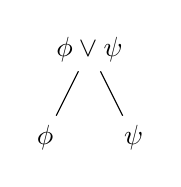
\begin{tikzpicture}[scale=0.75]
    \node {$\phi\lor\psi$}
        child {node {$\phi$}}
        child {node {$\psi$}};
    \end{tikzpicture}
    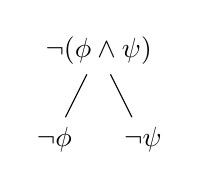
\begin{tikzpicture}[scale=0.75]
    \node {$\lnot(\phi\land\psi)$}
        child {node {$\lnot\phi$}}
        child {node {$\lnot\psi$}};
    \end{tikzpicture}
    \begin{tikzpicture}[scale=0.75]
    \node {$\lnot\lnot\phi$}
        child {node {$\phi$}};
    \end{tikzpicture}
    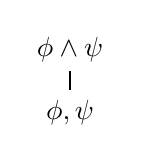
\begin{tikzpicture}[level distance=8mm]
    \node {$\phi\land\psi$}
        child {node {$\phi, \psi$}};
    \end{tikzpicture}  
    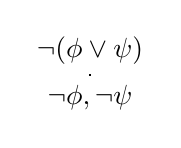
\begin{tikzpicture}[level distance=8mm,scale=0.75]
    \node {$\lnot(\phi\lor\psi)$}
        child {node {$\lnot\phi, \lnot\psi$}};
   \end{tikzpicture}
    Les règles
\end{frame}


\begin{frame}{Exemple}
    \textbf{Formule:} $a \Rightarrow (b \Rightarrow a)$

    \begin{center}
        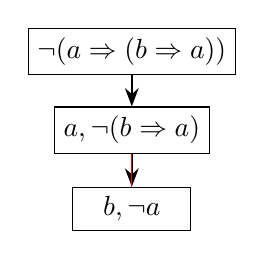
\begin{tikzpicture}[
            every node/.style={draw, minimum width=1.5cm, align=center},
            every arrow/.style={thick,->,>=Stealth}
        ]
        \node (root) at (0,0) {$\lnot(a \Rightarrow (b \Rightarrow a))$};
        \pause
        \node (not_b_a) at (0,-1) {$a, \lnot(b \Rightarrow a)$};
        \draw[every arrow] (root) -- (not_b_a);
        \pause
        \node (b) at (0,-2) {$b, \lnot a$};
        \draw[every arrow] (not_b_a) -- (b);
        \pause
        \draw[red] (not_b_a) -- (b);
        \end{tikzpicture}
    \end{center}
\end{frame}

\begin{frame}{Implémentation}
    Le code
\end{frame}

\begin{frame}{Ce qui est à faire}
    Mon but sur le long terme
    \begin{itemize}[<+->]
        \item Implémenter la méthode entière en logique propositionelle
        \item Trouver et prouver des optimisations pour les (?)
        \item Implémenter et commenter les résultats de l'optimisation
        \item Faire de même en logique du première ordre OU continuer à trouver des optimisations dans la logique propositionelle
    \end{itemize}
    \pause
    Sur le court terme :
    \begin{itemize}[<+->]
        \item Finir l'implémentation complète de la méthode des tableaux en logique propositionelle
        \item Faire les preuves de correction, terminaison
        \item Commencer la recherche de d'optimisation
    \end{itemize}
\end{frame}
\end{document}